\renewcommand\thesection{XIII}
\section{Circuits à Courant Alternatif: Déphasage, Représentation de Fresnel, Phaseurs, et Réactance}

\begin{multicols*}{2}
    \subsection{Source de f.é.m. alternative}
    
    \begin{center}
        \begin{circuitikz}
            \draw (0,0) to [vsourcesin] (3, 0);
        \end{circuitikz}
    \end{center}
    
    \paragraph{Exemple}
    Centrale Électrique
    
    \subsection{Circuits AC simples}
    
    \subsubsection{Circuits à une résistance}
    
    \begin{center}
        \begin{circuitikz}
            \draw (0, 0) to [vsourcesin = $v$] (3, 0) to (3, -1.5) to [R = $R$] (0, -1.5) to (0, 0);
        \end{circuitikz}
    \end{center}
    
    \begin{align*} 
        v_R &= v &\text{Kirchhoff} \\
        v_R &= Ri &\text{Ohm} \\
        \Rightarrow v &= Ri \\
        &= \frac{v_{0R}}{R} \sin(\omega T + \varphi) \\
        &= i_0 \sin(\omega t + \varphi) \\
        \text{Avec} &\quad v_{0R} = i_0 R
    \end{align*}
    
    \begin{center}
        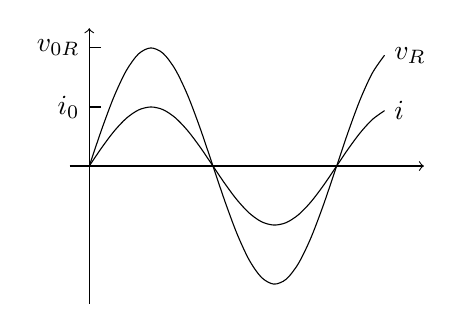
\begin{tikzpicture}[scale=0.5,domain=0:7.5,smooth]
            \draw[->] (0, -3.5) to (0, 3.5);
            \draw[->] (-0.5, 0) to (8.5, 0);
            
            \draw (0.3, 3) to (0, 3) node[left] {$v_{0R}$};
            \draw (0.3, 1.5) to (0, 1.5) node[left] {$i_0$};
            
            \draw plot (\x, {3* sin(\x r)}) node[right] {$v_R$};
            \draw plot (\x, {1.5 *sin(\x r)}) node[right] {$i$};
        \end{tikzpicture}
    \end{center}
    
    $i$ et $v_R$ ont la même fréquence $f = \frac{\omega}{2 \pi}$ et sont en phase.
    
    \subsubsection{Circuits à un condensateur}
    \begin{center}
        \begin{circuitikz}
            \draw (0, 0) to [vsourcesin = $v$] (3, 0) to (3, -1.5) to [C = $C$] (0, -1.5) to (0, 0);
        \end{circuitikz}
    \end{center}
    
    \begin{align*}
        v_C &= v &\text{Kirchhoff} \\
        v_C &= \frac{q}{C} &\text{Chap X} \\
        i &= \frac{dq}{dt} & q \to i \\
        \Rightarrow dq &= idt = i_0 \sin(\omega t) dt \\
        \Leftrightarrow q &= \frac{-i_0}{\omega} \cos(\omega t) = \frac{i_0}{\omega}\sin(\omega t-\frac{\pi}{2}) \\
        \Rightarrow v &= \frac{i_0}{\omega C} \sin(\omega t - \frac{\pi}{2}) = v_{0C} \sin(\omega t - \frac{\pi}{2}) \\
        \text{Avec} &\quad v_{0C} = \frac{i_0}{\omega C}
    \end{align*}
    
    \begin{center}
        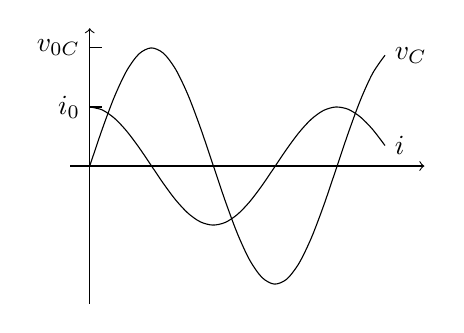
\begin{tikzpicture}[scale=0.5,domain=0:7.5,smooth]
            \draw[->] (0, -3.5) to (0, 3.5);
            \draw[->] (-0.5, 0) to (8.5, 0);
            
            \draw (0.3, 3) to (0, 3) node[left] {$v_{0C}$};
            \draw (0.3, 1.5) to (0, 1.5) node[left] {$i_0$};
            
            \draw plot (\x, {3* sin(\x r)}) node[right] {$v_C$};
            \draw plot (\x, {1.5 *sin((\x + pi/2) r)}) node[right] {$i$};
        \end{tikzpicture}
    \end{center}
    
    $i$ et $v_C$ ont la même fréquence $f = \frac{\omega}{2\pi}$ mais ne sont pas en phase. Il y a un déphasage de $\varphi = \frac{\pi}{2}$. $vC$ est en retard par rapport à $i$ d'un angle $\frac{\pi}{2}$.
    
    \subsubsection{Circuits à un inducteur}
    
    \paragraph{Note -- Loi de Lenz et Loi d'Ohm}
    Une bobine s'oppose au passage du courant alternatif. Ce comportement est similaire à une résistance qui s'oppose au passage du courant continu.
    
    \begin{center}
        Ohm : $V_A -V_B = RI$
        
        Lenz : $V_A - V_B = L \frac{di}{dt}$
    \end{center}
    
    \begin{center}
        \begin{circuitikz}
            \draw (0, 0) to [vsourcesin = $v$] (3, 0) to (3, -1.5) to [L = $L$] (0, -1.5) to (0, 0);
        \end{circuitikz}
    \end{center}
    
    \begin{align*}
        v &= L\omega i_0 \cos(\omega t) \\
        &= L\omega i_0 \sin(\omega t + \frac{\pi}{2}) \\
        &= v_{0L} \sin(\omega t + \frac{\pi}{2}) \\
        \text{Avec} &\quad v_{0L} = i_0\omega L
    \end{align*}
    
    \begin{center}
        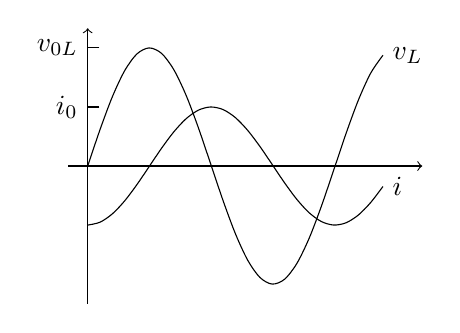
\begin{tikzpicture}[scale=0.5,domain=0:7.5,smooth]
            \draw[->] (0, -3.5) to (0, 3.5);
            \draw[->] (-0.5, 0) to (8.5, 0);
            
            \draw (0.3, 3) to (0, 3) node[left] {$v_{0L}$};
            \draw (0.3, 1.5) to (0, 1.5) node[left] {$i_0$};
            
            \draw plot (\x, {3* sin(\x r)}) node[right] {$v_L$};
            \draw plot (\x, {1.5 *sin((\x - pi/2) r)}) node[right] {$i$};
        \end{tikzpicture}
    \end{center}
    
    $i$ et $v_L$ ont la même fréquence $f = \frac{\omega}{2\pi}$ mais ne sont pas en phase. Il y a un déphasage de $\varphi = \frac{\pi}{2}$. $v_L$ devance $i$ d'un angle $\frac{\pi}{2}$.
    
    \subsection{Circuit AC RLC en série}
    
    \paragraph{Circuit RLC} Circuit comportant une résistance $R$, un inducteur $L$, et un capaciteur $C$ en série.
    
    \begin{center}
        \begin{circuitikz}
            \draw (0,0) to [vsourcesin = $v$] (0, 2) to [R = $R$] (3, 2) to [C = $C$] (3, 0) to [L = $L$] (0,0);
        \end{circuitikz}
    \end{center}
    
    Un même courant $i$ circule dans le circuit.
    \[ i_R = i_C = i_L = i = i_0 \sin(\omega t) \]
    
    D'où on trouve les tensions suivantes:
    \begin{align*}
        v_R &= R i_0 \sin(\omega t) = v_{0R} \sin(\omega t) \\
        v_C &= \frac{1}{\omega C} i_0 \sin(\omega t - \frac{\pi}{2}) = v_{0C} \sin(\omega t - \frac{\pi}{2}) \\
        v_L &= \omega L i_0 \sin(\omega t + \frac{\pi}{2}) = v_{0L} \sin(\omega t + \frac{\pi}{2})
    \end{align*}
    
    Par la loi des Mailles:
    \[v_{\text{source}} = v_R + v_C + v_L\]
    
    \subsection{Représentation de Fresnel}
    
    \paragraph{Vecteur de Fresnel}
    Une tension $v = v_0 \sin(\omega t + \varphi)$ est représentée dans le plan $Oxy$ par un vecteur de longueur égale à l'amplitude de la tension $v_0$ faisant un angle $\omega t + \varphi$ avec l'axe $Ox$.
    
    \begin{center}
        \begin{tikzpicture}
            \draw[->] (0, 0) node[left] {0} to (4, 0) node[below] {$x$};
            \draw[->] (0, 0) to (0, 3) node[left] {$y$};
            \draw[->] (0, 0) -- (3, 2) node[pos=0.5, above, sloped] {$v_0$};
            \draw[dotted] (0, 2) node[left] {$v_y$} to (3, 2);
            \draw[->] (2, 0) arc (0:34:2) node[pos=0.6,right] {$\omega t + \varphi$};
        \end{tikzpicture}
    \end{center}
    
    La tension intantanée est donnée par $v_y$:
    \[ v_y = v_0 \sin(\omega t + \varphi) \]
    
    $v_{\text{source}}$ devient une relation entre les composantes $y$ des vecteurs représentant les trois différentes tensions instantanées:
    \[ v_y = V_{Ry} + V_{Cy} + v_{Ly} \]
    
    \paragraph{Trouver la tension instantanée}
    Revient à faire la somme des vecteurs $v_R$, $v_C$, et $v_L$ et de projeter la résultante $v_0$ sur l'axe $Oy$.
    
    \begin{center}
        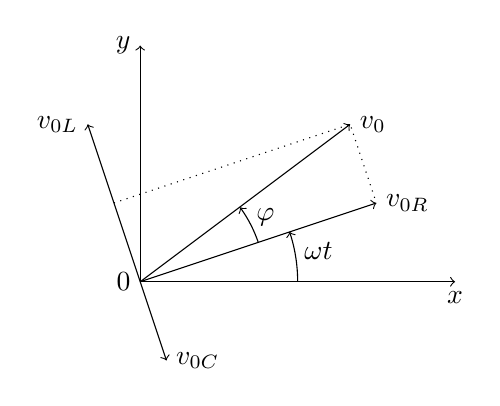
\begin{tikzpicture}
            \draw[->] (0, 0) node[left] {0} to (4, 0) node[below] {$x$};
            \draw[->] (0, 0) to (0, 3) node[left] {$y$};
            \draw[->] (0, 0) -- (3, 1) node[right] {$v_{0R}$};
            \draw[->] (0, 0) -- (-2/3, 2) node[left] {$v_{0L}$};
            \draw[->] (0, 0) -- (1/3, -1) node[right] {$v_{0C}$};
            \draw[->] (2, 0) arc (0:18.5:2) node[pos=0.6,right] {$\omega t$};
            
            \draw[dotted] (-1/3, 1) -- (-1/3 + 3, 2) -- (3, 1);
            \draw[->] (0, 0) -- (-1/3 + 3, 2) node[right] {$v_0$};
            \draw[->] (1.5, 0.5) arc (19:36:1.7) node[pos=0.7,right] {$\varphi$};
        \end{tikzpicture}
    \end{center}
    
    Avec $v_0$ l'amplitude de $v$ donnée par:
    \[ v_0 = \sqrt{(v_{0L} - v_{0C})^2 + v_{O_R}^2} \]
    
    Et $\varphi$ l'angle que $v$ fait avec $i$ donné par:
    \[ \cos \varphi = \frac{v_{0R}}{v_0} \qquad \text{ou} \qquad \tan \varphi = \frac{v_{0L}-v_{0C}}{v_{0R}}  \]
    
    \subsection{Phaseurs}
    
    \paragraph{Représentation dans le plan complexe}
    On représente la tension par un point complexe qui est l'extrémité du vecteur de Fresnel
    \[ z = x + jy \qquad \text{où} \quad j = \sqrt{-1} \]
    
    \begin{center}
        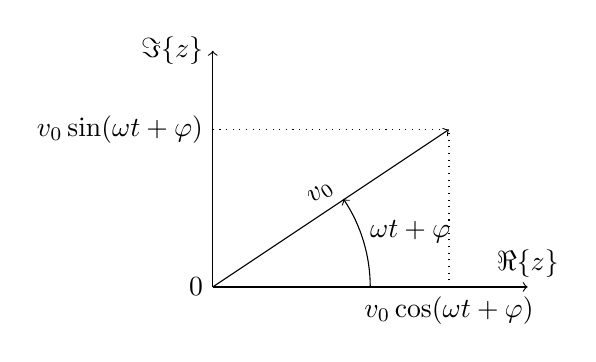
\begin{tikzpicture}
            \draw[->] (0, 0) node[left] {0} to (4, 0) node[above] {$\Re \{z\}$};
            \draw[->] (0, 0) to (0, 3) node[left] {$\Im \{z\}$};
            \draw[->] (0, 0) -- (3, 2) node[pos=0.5, above, sloped] {$v_0$};
            \draw[dotted] (0, 2) node[left] {$v_0 \sin(\omega t + \varphi)$} to (3, 2);
            \draw[dotted] (3, 0) node[below] {$v_0 \cos(\omega t + \varphi)$} to (3, 2);
            \draw[->] (2, 0) arc (0:34:2) node[pos=0.6,right] {$\omega t + \varphi$};
        \end{tikzpicture}
    \end{center}
    \begin{align*}
        \Rightarrow z &= v_0[\cos(\omega t + \varphi) + j \sin(\omega t + \varphi)] \\
        &= v_0 e^{j(\omega t + \varphi)} = v_0 e^{j\omega t} e^{j \varphi}
    \end{align*}
    
    La tension instantanée est donnée par:
    \[v = \Im \{ v_0 e^{j(\omega t + \varphi)} \} \]
    
    \paragraph{Phaseur} Dans la représentation de Fresnel, la relation de phase entre les différentes tensions reste constante. On peut donc travailler avec le phaseur $\tilde{v}$: un nombre complexe associé à une tension instantanée d'amplitude $v_0$ et de phase $\varphi$.
    \[ \tilde{v} = v_0 e^{j(\omega t + \varphi)} \]
    
    \subsubsection{Circuit RLC}
    
    On a les phaseurs suivants:
    \begin{align*}
        \tilde v_R &= v_{0R} \qquad &\text{car} \quad \varphi = 0 \\
        \tilde v_C &= v_{0C} e^{-j\frac{\pi}{2}} = -v_{0C}j \qquad &\text{car} \quad \varphi = \frac{-\pi}{2}  \\
        \tilde v_L &= v_{0L} e^{j \frac{\pi}{2}} = v_{0L}j \qquad &\text{car} \quad \varphi = \frac{\pi}{2} \\
        \Rightarrow \tilde v &= \tilde v_R + \tilde v_C + \tilde v_L \\
        &= v_{0R} + (v_{0L} - v_{0C}) j
    \end{align*}
    
    On en déduit l'amplitude $v_0$ et la phase $\varphi$:
    \begin{align*}
        v_0 = |\tilde v| = \sqrt{ v_{0R}^2 + (v_{0L} - v_{0C})^2 } \\
        \cos \varphi = \frac{\Re \{\tilde v\}}{|\tilde v|} = \frac{v_{0R}}{v_0}
    \end{align*}
    
    \subsection{Réactance}
    
    \subsubsection{Réactance Capacitive}
    Quantifie la manière dont un condensateur freine le courant. $X_C$ exprimé en Ohm ($\Omega$).
    \begin{align*}
        X_C &= \frac{v_{0C}}{i_0} \\
        X_C &= \frac{1}{\omega C} \qquad \text{avec} \quad i_0 = \omega C v_{0C}
    \end{align*}
    
    $X_C$ diminue lorsque $\omega$ augmente. Plus la fréquence est frande, moins les charges ont le temps de s'accumuler sur les armatures du condensateur, et moins ce dernier freine l'accès aux électrons.
    
    \begin{center}
        \begin{tikzpicture}[scale=0.5,domain=0.2:5,smooth]
            \draw plot (\x, {1/\x});
            \draw[->] (0,0) -- (0,5.5) node[above] {$X_C$};
            \draw[->] (0,0) -- (5.5,0) node[right] {$\omega$};
        \end{tikzpicture}
    \end{center}
    
    \paragraph{Courant DC}
    Pour un courant DC: $\omega = 0$. Ceci mène à une réactance capacitive qui tend vers $+\infty$.
    
    \subsubsection{Réactance Capacitive}
    Quantifie la manière dont un inducteur freine le courant. $X_L$ exprimé en Ohm ($\Omega$).
    
    \begin{align*}
        X_C &= \frac{v_{0L}}{i_0} \\
        X_C &= \omega L \qquad \text{avec} \quad i_0 = \frac{v_{0L}}{\omega L}
    \end{align*}
    
    \begin{center}
        \begin{tikzpicture}[scale=0.5,domain=0.2:5,smooth]
            \draw plot (\x, {\x});
            \draw[->] (0,0) -- (0,5.5) node[above] {$X_L$};
            \draw[->] (0,0) -- (5.5,0) node[right] {$\omega$};
        \end{tikzpicture}
    \end{center}
    
\end{multicols*}